\chapter{Zkouškové otázky}

\begin{enumerate}
	\item Uveďte základní skupiny konstitutivních modelů látek s~ohledem na směrovou závislost vlastností, na velikost a~vratnost deformací a~jejich časovou závislost?
	\item Jak jsou definovány ideálně tuhá látka, ideální kapalina a~ideální plyn?
	\item Co je to kulová složka tenzoru a~deviátor tenzoru? Uveďte příklad.
	\item Jak je definován hyperelastický materiál?
	\item Jaká je základní struktura funkcí popisujících měrnou energii napjatosti hyperelastických materiálů, jaké matematické funkce se nejčastěji používají?
	\item Jak je definován objemový modul pružnosti?
	\item Jaké znáte elastické konstanty lineárně pružného izotropního homogenního materiálu?
	\item Jaké znáte definice tenzoru deformace (nejen přetvoření) při velkých deformacích?
	\item Co je polární dekompozice tenzoru deformačního gradientu?
	\item Jaké znáte definice tenzoru napětí při velkých deformacích?
	\item Jak se vzájemně přepočítavají smluvní a~skutečné hodnoty tenzorů přetvoření a~napětí?
	\item Co jsou modifikované (redukované) invarianty tenzoru deformace?
	\item Co jsou to modifikovaná (redukovaná) poměrná protažení $\bar{\lambda}_i$?
	\item Co jsou to energeticky konjugované tenzory? Uveďte příklad.
	\item Uveďte příklad konstitutivního modelu hyperelastického materiálu a~vysvětlete význam veličin.
	\item Určete fyzikální rozměry jednotlivých parametrů konstitutivního modelu zadaného rovnicí pro měrnou deformační energii.
	\item Pro konstitutivní model zadaný rovnicí pro měrnou deformační energii určete, jaký typ chování popisuje.
	\item Jaký typ modelu použijete pro popis zadané tahové křivky materiálu?
	\item Čím se model Arruda-Boyce principiálně liší od fenomenologických polynomických konstitutivních modelů?
	\item Jaký model dostaneme, pokud v~se modelu Arruda-Boyce limitní protažení řetězců $\lambda_L$ blíží nekonečnu?
	\item Jaké materiálové zkoušky jsou potřebné pro úplný popis mechanického chování izotropního hyperelastického málo stlačitelného materiálu?
	\item Co je označováno termínem \enquote{pure shear} (čistý smyk)?
	\item Uveďte mechanické zkoušky ekvivalentní zadaných typům zkoušek pro hyperelastický nestlačitelný materiál.
	\item Jaká je základní struktura konstitutivních modelů anizotropního hyperelastického materiálu, s~jakými veličinami tyto modely pracují?
	\item Rozepište danou tenzorovou rovnici, ve které je použito Einsteinovo sčítací pravidlo.
	\item Převeďte dané složky tenzoru druhého řádu na jednoindexovou notaci.
	\item Proveďte zadanou tenzorovou operaci (tenzorový součin vektorů, úžení tenzorů 2. řádu).
	\item Vyjádřete měrnou energii napjatosti lineárně elastického materiálu pomocí napětí.
	\item Co je to entropická elasticita, jaká je její základní energetická veličina, kdy se uplatňuje?
	\item Co je to perzistentní délka vlákna?
	\item Jaké další (pseudo)invarianty deformačního denzoru se používají pro popis anizotropního hyperelastického materiálu (oproti izotropnímu), uveďte definici a~fyzikální význam aspoň jednoho z~nich.
	\item Co je Mullinsův efekt, vysvětlete na tahovém diagramu.
	\item Jaké typy chování materiálu lze popsat jeho viskoelastickým modelem?
	\item Vyjádřete Newtonův zákon viskozity pomocí úhlového přetvoření.
	\item Které materiálové charakteristiky se používají v~lineárně viskoelastických modelech? Kolik z~nich je nezávislých?
	\item Nakreslete reologická schemata aspoň tří nejjednodušších reologických modelů a~popište jejich materiálové charakteristiky.
	\item Napište maticový tvar tenzoru napětí pro ideální kapalinu podle konvencí mechaniky těles.
	\item Jaké základní prvky se používají pro tvorbu reologických modelů?
	\item Co je to časová konstanta materiálu (relaxační doba, retardační doba), jak se určí?
	\item Popište chování Maxwellova (Voigtova, Kelvinova) modelu viskoelastické látky při skokové změně napětí nebo deformace.
	\item Co je to komplexní modul pružnosti?
	\item Nakreslete příklad diskrétního a~spojitého spektra relaxačních funkcí, popište osy.
	\item Jaké typy konstitutivních modelů jsou potřebné pro úplný popis chování pružně-plastického materiálu až do porušení při monotonním a~cyklickém zatěžování?
	\item Jaký výsledek dostanete, jestliže v~podmínce plasticity Mohr-Coulomb (Drucker-Prager) zadané rovnicí pro redukované napětí použijete stejnou mez pružnosti pro tah a~tlak ($m=1$)?
	\item Co je faktor triaxiality napětí? Jakých nabývá hodnot?
	\item Co je Lodeho parametr nebo úhel? V~jakém rozmezí se pohybují jeho hodnoty?
	\item Určete faktor triaxiality napětí pro zadanou napjatost.
\end{enumerate}

%\section*{Otázky ke zkoušce z~předmětu Konstitutivní vztahy materiálu}\addcontentsline{toc}{section}{Otázky ke zkoušce z~předmětu Konstitutivní vztahy materiálu}
%
%\subsection{Uveďte základní skupiny konstitutivních modelů látek s~ohledem na směrovou závislost vlastností, na velikost a~vratnost deformací a~jejich časovou závislost?}
%%S~jakými konstitutivními modely jsme se již setkali? 
%%\begin{itemize}
%%	\item Ideálně tuhý materiál
%%	\item Lineárně elastický materiál (izotropní nebo anizotropní -- vláknové kompozity) -- Hookův zákon
%%	\item Elasticko-plastický materiál (ideálně, tj. bez zpevnění, anebo se zpevněním)
%%	\item Tuho-plastický materiál
%%\end{itemize}
%%
%%Jaké další modely budou probírány v~předmětu „Konstitutivní vztahy materiálu“?
%%\begin{itemize}
%%	\item Viskoelastické modely materiálu (napětí a~deformace jsou mj. funkcí času) s~malými deformacemi i~s~velkými deformacemi (visko-hyperelastické)
%%	\item Hyperelastické modely materiálu  (materiál vykazující velká elastická přetvoření) izotropní a~anizotropní
%%	\item Elasticko-plastické modely materiálu
%%	\item Modely porušení
%%\end{itemize}
%
%Tuhý materiál
%\begin{itemize}
%	\item nedeformovatelný
%\end{itemize}
%
%Elastický materiál
%\begin{itemize}
%	\item nezávislý na rychlosti zatěžování
%	\item bez hystereze (nulová disipace)
%	\item lineární (Hookeův zákon) nebo nelineární
%	\item anizotropní (vláknové kompozity), ortotropní, příčně izotropní nebo izotropní (ocel)
%\end{itemize}
%
%(Hyperelastický materiál)
%\begin{itemize}
%	\item materiál vykazující velká elastická přetvoření
%\end{itemize}
%
%Visko-elastický materiál
%\begin{itemize}
%	\item napěťově-deformační odezva je závislá na rychlosti zatěžování
%	\item s~malými deformacemi i~s~velkými deformacemi
%\end{itemize}
%
%Elasto-plastický materiál
%\begin{itemize}
%	\item bez zpevnění nebo se zpevněním (izotropní nebo kinematické)
%\end{itemize}
%
%Elasto-visko-plastický materiál
%
%Modely porušení
%
%\subsection{Jak jsou definovány ideálně tuhá látka, ideální kapalina a~ideální plyn?}
%Ideálně tuhá látka
%\begin{itemize}
%	\item Nekonečně velký odpor proti deformaci.
%	\item Deformace je pro daný problém nepodstatná.
%\end{itemize}
%
%Ideální kapalina
%\begin{itemize}
%	\item Nulová viskozita, tj. žádné vnitřní tření, nulový odpor proti změně tvaru.
%	\item Objemová nestlačitelnost, tj. nekonečně velký odpor proti změně objemu.
%\end{itemize}
%
%Ideální plyn
%\begin{itemize}
%	\item Nulová viskozita, tj. žádné vnitřní tření, nulový odpor proti změně tvaru
%	\item Značná objemová stlačitelnost a~současně rozpínavost, tj. schopnost vyplnit celý disponibilní prostor.
%	\item Odpor proti změně objemu je velmi malý a~řídí se stavovou rovnicí ideálního plynu.
%\end{itemize}
%
%\subsection{Co je to kulová složka tenzoru a~deviátor tenzoru? Uveďte příklad.}
%Kulová složka tenzoru -- Popisuje změnu objemu tělesa při zachování tvaru. Není schopna vyvolat trvalou plastickou deformaci.
%
%Deviátorová složka tenzoru -- Popisuje změnu tvaru tělesa bez změny objemu. Je schopen vyvolat trvalou plastickou deformaci.
%\begin{align*}
%	\bm{T} &= \bm{T}^\text{kul} + \bm{T}^\text{dev}\\
%	\bm{T}^\text{kul} &:= \frac{1}{3}(\bm{T} : \bm{1}) \bm{1}\\
%	\bm{T}^\text{dev} &:= \bm{T} - \bm{T}^\text{kul}
%\end{align*}
%\subsection{Jak je definován hyperelastický materiál?}
%Jako hyperelastické označujeme materiály vykazující konečná (tj. velká) vratná přetvoření.
%
%Materiál nazýváme hyperelastickým, pokud existuje elastická potenciální funkce $W$ (měrná deformační energie), která je skalární funkcí některého z~tenzorů přetvoření, resp. deformace a~jejíž parciální derivace podle některé složky přetvoření pak určuje odpovídající složku napětí, například:
%\begin{equation*}
%	\bm{S} = \frac{\partial W(\bm{E})}{\partial \bm{E}} = 2 \frac{\partial W(\bm{C})}{\partial \bm{C}},
%\end{equation*}
%kde
%\begin{description}
%	\item[$\bm{S}$] je 2.~Piolův-Kirchhoffův tenzor napětí
%	\item[$W$] je funkce měrné energie napjatosti na jednotku nedeformovaného objemu
%	\item[$\bm{E}$] je Greenův-Lagrangeův tenzoru přetvoření $\bm{E} = \frac{1}{2}(\bm{C} - \bm{1})$
%	\item[$\bm{C}$] je pravý Cauchyho-Greenův tenzor deformace
%\end{description}
%
%\subsection{Jaká je základní struktura funkcí popisujících měrnou energii napjatosti hyperelastických materiálů, jaké matematické funkce se nejčastěji používají?}
%U~všech hyperelastických konstitutivních modelů je stejně jako u~většiny ostatních třeba odděleně modelovat objemovou a~tvarovou (deviátorovou) složku deformace.
%Proto konstitutivní vztahy sestávají ze dvou částí:
%\begin{itemize}
%	\item Vliv změny objemu na energii napjatosti popisují nejčastěji třetím invariantem tenzoru gradientu deformace $J$ a~konstantou popisující objemovou změnu (objemový modul pružnosti nebo jiná konstanta z~něj odvozená). Kromě pěnových gum je změna objemu malá oproti změně tvaru a~většinou vystačíme s~jejím lineárním popisem.
%	\item Vliv tvarové změny se popisuje nejčastěji pomocí modifikovaných invariantů některého z~tenzorů přetvoření. Modifikace má za cíl právě oddělení tvarové změny (deviátorové složky tenzoru) od změny objemové (kulová složka tenzoru).
%\end{itemize}
%
%Nejčastěji se používají polynomické funkce.
%
%\subsection{Jak je definován objemový modul pružnosti?}
%Modul objemové pružnosti je definován podobně jako v~hydromechanice
%\begin{equation}
%K = \frac{\sigma_s}{e},
%\end{equation}
%kde
%\begin{itemize}
%	\item[$\sigma_s$] je střední napětí,
%	\item[$e$] je poměrná změna objemu.
%\end{itemize}
%
%Pro tyto veličiny byly v~PPII odvozeny vztahy
%\begin{align}
%	\sigma_s &= \frac{\sigma_1 + \sigma_2 + \sigma_3}{3},\\
%	e &= \varepsilon_1 + \varepsilon_2 + \varepsilon_3,
%\end{align}
%do nichž dosadíme z~Hookova zákona a~dostaneme:
%\begin{equation}\begin{split}
%	e
%	&= \varepsilon_1 + \varepsilon_2 + \varepsilon_3
%	= \frac{1}{E} \left[\sigma_1 - \mu(\sigma_2 + \sigma_3)\right]
%	+ \frac{1}{E} \left[\sigma_2 - \mu(\sigma_1 + \sigma_3)\right]
%	+ \frac{1}{E} \left[\sigma_3 - \mu(\sigma_1 + \sigma_2)\right]\\
%	&= \frac{1}{E} \left[\sigma_1 (1-2\mu) + \sigma_2 (1-2\mu) + \sigma_3 (1-2\mu)\right]
%	= \frac{1-2\mu}{E} \left(\sigma_1 + \sigma_2 + \sigma_3\right)
%\end{split}\end{equation}
%
%Dosazením do definičního vztahu pro $K$ dostaneme
%\begin{equation*}
%	K
%	= \frac{\sigma_s}{e}
%	= \frac{\frac{\sigma_1 + \sigma_2 + \sigma_3}{3}}{\frac{(1-2\mu) (\sigma_1 + \sigma_2 + \sigma_3)}{E}}
%	= \frac{E}{3 (1-2\mu)}
%\end{equation*}
%
%\subsection{Jaké znáte elastické konstanty lineárně pružného izotropního homogenního materiálu?}
%Modul pružnosti v~tahu $E\:[\si{\pascal}]$
%
%Modul pružnosti ve smyku $G = \frac{E}{2(1+\mu)}\:[\si{\pascal}]$
%
%Modul objemové pružnosti $K = \frac{E}{3 (1-2\mu)}\:[\si{\pascal}]$
%
%Lamého konstanta lambda $\lambda = \frac{E \mu}{(1+\mu) (1-2\mu)} = K - \frac{2}{3} G\:[\si{\pascal}]$
%
%Poissonovo číslo $\mu = \frac{3K - 2G}{6K + 2G}\:[-]$ (dává obvyklou představu o~stlačitelnosti materiálu)
%
%\subsection{Jaké znáte definice tenzoru deformace (nejen přetvoření) při velkých deformacích?}
%\subsubsection{Tenzor deformačního gradientu}
%Složkami tenzoru deformačního gradientu $\bm{F}$ jsou poměrná protažení. Obecně je lze zapsat ve tvaru:
%\begin{equation*}
%	\bm{F} := \frac{\partial \bm{x}}{\partial \bm{X}}
%	\quad\Leftrightarrow\quad
%	F_{iJ}  := \frac{\partial x_i}{\partial X_J}
%\end{equation*}
%
%Poměrná protažení $\{\lambda_i\}_{i=1..3}$ jsou vlastní čísla tenzoru $\bm{F}$ získaná spektrální dekompozicí:
%\begin{equation*}
%	\bm{F} = \sum_{i=1}^{3} \lambda_i \, \bm{n}_i \otimes \bm{N}_i
%\end{equation*}
%
%Maticové zápisy složek v~obecném a~hlavním souřadnicovém systému jsou:
%\begin{equation*}
%	\bm{F} = \left(\begin{matrix}
%	\frac{\partial x_1}{\partial X_1} & \frac{\partial x_1}{\partial X_2} & \frac{\partial x_1}{\partial X_3}\\
%	\frac{\partial x_2}{\partial X_1} & \frac{\partial x_2}{\partial X_2} & \frac{\partial x_2}{\partial X_3}\\
%	\frac{\partial x_3}{\partial X_1} & \frac{\partial x_3}{\partial X_2} & \frac{\partial x_3}{\partial X_3}
%	\end{matrix}\right)
%	\quad\text{respektive}\quad
%	\bm{F} = \left(\begin{matrix}
%		\lambda_1 & 0 & 0\\
%		0 & \lambda_2 & 0\\
%		0 & 0 & \lambda_3
%	\end{matrix}\right)
%\end{equation*}
%
%Invarianty v~obecném a~hlavním souřadnicovém systému:
%\begin{equation*}
%	\begin{aligned}
%		I_1(\bm{F}) &= \mathrm{tr}(\bm{F})\\
%		I_2(\bm{F}) &= \frac{1}{2} \left[\mathrm{tr}(\bm{F})^2 - \mathrm{tr}(\bm{F}^2)\right]\\
%		I_3(\bm{F}) &= \det(\bm{F})
%	\end{aligned}
%	\quad\text{respektive}\quad
%	\begin{aligned}
%		I_1(\bm{F}) &= \lambda_1 + \lambda_2 + \lambda_3\\
%		I_2(\bm{F}) &= \lambda_1 \lambda_2 + \lambda_2 \lambda_3 + \lambda_3 \lambda_1\\
%		I_3(\bm{F}) &= \lambda_1 \lambda_2 \lambda_3 = J
%	\end{aligned}
%\end{equation*}
%
%\subsubsection{Cauchyho-Greenův tenzor deformace}
%Cauchyho\footnote{Augustin-Louis Cauchy (1789---1857)}-Greenův\footnote{George Green (1793---1841)} tenzor deformace:
%\begin{equation*}
%	\bm{C} := \bm{F}^T \!\cdot\! \bm{F}
%	\quad\Leftrightarrow\quad
%	C_{IJ} := F_{kI} F_{kJ} = \frac{\partial x_k}{\partial X_I} \frac{\partial x_k}{\partial X_J}
%\end{equation*}
%
%Složkami tenzoru v~hlavním souřadnicovém systému jsou kvadráty poměrných protažení:
%\begin{equation*}
%	\bm{C} = \left(\begin{matrix}
%		\lambda_1^2 & 0 & 0\\
%		0 & \lambda_2^2 & 0\\
%		0 & 0 & \lambda_3^2
%	\end{matrix}\right)
%\end{equation*}
%
%Invarianty v~obecném a~hlavním souřadnicovém systému:
%\begin{equation*}
%	\begin{aligned}
%		I_1(\bm{C}) &= \mathrm{tr}(\bm{C})\\
%		I_2(\bm{C}) &= \frac{1}{2} \left[\mathrm{tr}(\bm{C})^2 - \mathrm{tr}(\bm{C}^2)\right]\\
%		I_3(\bm{C}) &= \det(\bm{C})
%	\end{aligned}
%	\quad\text{respektive}\quad
%	\begin{aligned}
%	I_1(\bm{C}) &= \lambda_1^2 + \lambda_2^2 + \lambda_3^2\\
%	I_2(\bm{C}) &= \lambda_1^2 \lambda_2^2 + \lambda_2^2 \lambda_3^2 + \lambda_3^2 \lambda_1^2\\
%	I_3(\bm{C}) &= \lambda_1^2 \lambda_2^2 \lambda_3^2 = J^2
%	\end{aligned}
%\end{equation*}
%
%\subsubsection{Fingerův tenzor deformace}
%Fingerův\footnote{Josef Finger (1841--1925)} tenzor deformace:
%\begin{equation*}
%	\bm{B} := \bm{F} \!\cdot\! \bm{F}^T
%	\quad\Leftrightarrow\quad
%	B_{IJ} := F_{Ik} F_{Jk} = \frac{\partial X_I}{\partial x_k} \frac{\partial X_J}{\partial x_k}
%\end{equation*}
%
%\subsubsection{Smluvní přetvoření (pro malé deformace)}
%\begin{equation*}
%	\bm{\varepsilon} := \tfrac{1}{2} \left( \nabla\bm{u} + \nabla^T\bm{u} \right)
%	\quad\Leftrightarrow\quad
%	\varepsilon_{IJ} := \frac{1}{2} \left( \frac{\partial u_i}{\partial X_J} + \frac{\partial u_j}{\partial X_I} \right)
%\end{equation*}
%
%\subsubsection{Greenův-Lagrangeův tenzor přetvoření}
%Přetvoření (poměrná deformace) je vztažena k~původním (nedeformovaným) rozměrům, ale je respektováno i~natáčení elementu. Nedostatkem je, že aktuální rozměry již mohou být v~průběhu procesu zatěžování významně odlišné.
%\begin{equation*}
%	\bm{E} = \frac{1}{2}\left(\bm{C} - \bm{1}\right)
%	\quad\text{nebo}\quad
%	E_{ij} = \frac{1}{2} \left[ \frac{\partial u_i}{\partial X_j} + \frac{\partial u_j}{\partial X_i} + \frac{\partial u_k}{\partial X_j} \frac{\partial u_k}{\partial X_i} \right]
%\end{equation*}
%
%\subsubsection{Almansiho-Hamelův tenzor přetvoření}
%Změny délek jsou vztahovány ke konečným (deformovaným) hodnotám délek. Nedostatkem je, že aktuální od nich mohou být v~průběhu procesu zatěžování ještě podstatně odlišné.
%\begin{equation*}
%	\bm{A} = \frac{1}{2}\left(\bm{1} - \bm{B}^{-1}\right)
%	\quad\text{nebo}\quad
%	A_{ij} = \frac{1}{2} \left[ \frac{\partial u_i}{\partial x_j} + \frac{\partial u_j}{\partial x_i} - \frac{\partial u_k}{\partial x_j} \frac{\partial u_k}{\partial x_i} \right]
%\end{equation*}
%Praktické použití tohoto tenzoru je omezeno tím, že konečné (deformované) souřadnice obvykle předem neznáme.
%
%\subsubsection{Cauchyho (logaritmický) tenzor přetvoření}
%Cauchyho definice přetvoření je exaktnější v~tom, že infinitezimální přírůstek délky vztahuje vždy k~aktuální délce v~daném stádiu zatěžovacího procesu.
%
%Přetvoření úsečky o~původní délce $X_{i0}$, která se vlivem zatížení mění na aktuální hodnotu $X_i$ až dosáhne konečné (deformované) délky $x_{ik}$, určíme integrací přírůstků její délky $\diff x_i$ (viz obrázek):
%\begin{equation*}
%	E^C_{ij}
%	= \int\limits_{X_{i0}}^{x_{ik}} \frac{1}{x_i} \diff x_i
%	= \left. \ln(x) \right\rvert_{X_{i0}}^{x_{ik}}
%	= \ln(x_{ik}) - \ln(X_{i0})
%	= \ln\left(\frac{x_{ik}}{X_{i0}}\right)
%	= \ln(\lambda_i)
%\end{equation*}
%
%Souřadnice tohoto tenzoru jsou tedy rovny přirozeným logaritmům odpovídajících souřadnic tenzoru deformačního gradientu.
%\begin{equation*}
%	E^C_{ij} = \ln(F_{ij}) = \frac{1}{2} \ln(C_{ij})
%\end{equation*}
%
%\subsubsection{Tenzor protažení}
%\begin{equation*}
%	\bm{U} = \bm{R}^{-1} \!\cdot\! \bm{F}
%\end{equation*}
%
%\subsection{Co je polární dekompozice tenzoru deformačního gradientu?}
%I~v~nedeformovaném stavu elementu může mít matice definující tenzor deformačního gradientu $\bm{F}$ složky odlišné od jednotkové matice; je to dáno případnou rotací elementu v~důsledku velkých deformací tělesa. Polární dekompozicí tenzoru $\bm{F}$ lze tento rozložit na tenzor rotace $\bm{R}$ (vyjadřující rotaci tuhého tělesa) a~tenzor protažení $\bm{U}$ (popisující deformaci tělesa).
%\begin{equation*}
%	\bm{F} = \bm{R} \!\cdot\! \bm{U}
%\end{equation*}
%
%Tenzor protažení $\bm{U}$ lze určit ze vztahu:
%\begin{equation*}
%	\bm{U} = \bm{R}^{-1} \!\cdot\! \bm{F} = \bm{R}^T \!\cdot\! \bm{F}
%\end{equation*}
%využívajícího ortogonality tenzoru rotace $\bm{R}$, pro který se inverzní matice rovná matici transponované. Hlavní složky tenzoru $\bm{U}$ jsou hlavní poměrná protažení. Tento tenzor je vždy symetrický na rozdíl od tenzoru deformačního gradientu $\bm{F}$.
%
%
%\subsection{Jaké znáte definice tenzoru napětí při velkých deformacích?}
%\subsubsection{Cauchyho tenzor napětí}
%Cauchyho tenzor napětí je definován jako skutečná elementární síla $\bm{f}$ vztažená na skutečnou (tj. deformovanou) plochu elementu $\bm{s}$ podle vztahu:
%\begin{equation*}
%	\bm{\sigma} := \frac{\diff \bm{f}}{\bm{n} \diff S}
%\end{equation*}
%Pro hlavní napětí platí:
%\begin{equation*}
%	\sigma_i = \frac{\diff f_i}{\diff x_j \diff x_k}
%\end{equation*}
%
%\subsubsection{1.~Piolův-Kirchhoffův tenzor}
%1.~Piolův-Kirchhoffův tenzor napětí je definován jako skutečná elementární síla $\bm{f}$ vztažená na původní (tj. nedeformovanou) plochu elementu $\bm{S}$ podle vztahu (platí pro hlavní napětí):
%\begin{equation*}
%	\bm{P} := \frac{\diff \bm{f}}{\bm{N} \diff S}
%\end{equation*}
%Pro hlavní napětí platí:
%\begin{equation*}
%	P_i = \frac{\diff f_i}{\diff X_j \diff X_k}
%\end{equation*}
%
%\subsubsection{2.~Piolův-Kirchhoffův tenzor napětí}
%2.~Piolův-Kirchhoffův tenzor napětí je definován jako elementární síla $\bm{f}$ vztažená na původní (tj. nedeformovanou) plochu elementu. Tato síla $\bm{f}_0$ je však při přenášení na původní element změnění vůči skutečné síle $\bm{f}$ stejným poměrem jako elementární rozměr v~odpovídajícím směru.
%\begin{equation}
%	\diff \bm{f} = \bm{F} \!\cdot\! \bm{f}_0,
%\end{equation}
%takže napětí je
%\begin{equation}
%	\bm{S} := \frac{\diff \bm{f}_0}{\bm{N} \diff S}
%\end{equation}
%Pro hlavní napětí platí:
%\begin{equation}
%	S_i = \frac{\diff f_{0i}}{\diff X_j \diff X_k}
%\end{equation}
%Tento tenzor nemá jasný fyzikální význam, používá se proto, že je i~pro velká přetvoření symetrický a~je energeticky konjugovaný s~Green-Lagrangeovým tenzorem přetvoření.
%
%\subsection{Jak se vzájemně přepočítavají smluvní a~skutečné hodnoty tenzorů přetvoření a~napětí?}
%Nejvhodnější pro vzájemný přepočet tenzorů přetvoření jsou poměrná protažení $\lambda_i$, tedy složky tenzoru deformačního gradientu. V~hlavním souřadnicovém systému platí následující vztahy:
%
%Hlavní Cauchyho (skutečné) napětí lze vyjádřit pomocí PK1 napětí
%\begin{equation}
%	\sigma_i = \frac{\diff F_i}{\diff x_j \diff x_k}
%	= \frac{\diff F_i}{\lambda_j \diff X_j \lambda_k \diff X_k}
%	= \frac{P_i}{\lambda_j \lambda_k}
%\end{equation}
%
%Pro nestlačitelný materiál platí $\lambda_i\lambda_j\lambda_k=1$ a~tedy napětí jsou ve vztahu
%\begin{equation}
%	\sigma_i = \frac{P_i}{\lambda_j \lambda_k} = P_i \lambda_i
%\end{equation}
%
%Podobně lze vyjádřit 2.P.K. napětí
%\begin{equation}
%	S_i = \frac{\diff f_{0i}}{\diff X_j \diff X_k}
%	= \frac{\frac{\partial X_i}{\partial x_i} \diff F_i}{\diff X_j \diff X_k}
%	= \frac{\frac{1}{\lambda_i} \diff F_i}{\diff X_j \diff X_k}
%	= \frac{1}{\lambda_i} P_i
%\end{equation}
%
%Cauchyho napětí lze vyjádřit i~pomocí PK2 napětí
%\begin{equation}
%	\sigma_i = \frac{P_i}{\lambda_j \lambda_k}
%	= \frac{\lambda_i}{\lambda_j \lambda_k} S_i,
%\end{equation}
%nebo jednodušeji pro nestlačitelný materiál
%\begin{equation}
%	\sigma_i = \lambda_i P_i = \lambda_i^2 S_i.
%\end{equation}
%
%\subsection{Co jsou modifikované (redukované) invarianty tenzoru deformace?}
%Modifikované (redukované) invarianty Cauchy-Greenova tenzoru deformace se používají pro popis deviátorové složky deformace.
%
%Modifikované invarianty Cauchy-Greenova tenzoru deformace jsou dány
%\begin{align*}
%	\bar{I}_1(\bm{C})
%	&= \bar{\lambda}_1^2 + \bar{\lambda}_2^2 + \bar{\lambda}_3^2
%	= \left(\lambda_1^2 + \lambda_2^2 + \lambda_3^2\right) J^{-\frac{2}{3}}
%	= I_1 J^{-\frac{2}{3}}
%	= I_1 I_3^{-\frac{1}{3}}\\
%	\bar{I}_2(\bm{C})
%	&= \bar{\lambda}_1^2 \bar{\lambda}_2^2 + \bar{\lambda}_2^2 \bar{\lambda}_3^2 + \bar{\lambda}_1^2 \bar{\lambda}_3^2
%	= \left(\lambda_1^2 \lambda_2^2 + \lambda_2^2 \lambda_3^2 + \lambda_1^2 \lambda_3^2\right) J^{-\frac{4}{3}}
%	= I_2 J^{-\frac{4}{3}}
%	= I_2 I_3^{-\frac{2}{3}}
%\end{align*}
%
%\subsection{Co jsou to modifikovaná (redukovaná) poměrná protažení $\bar{\lambda}_i$?}
%U~smluvních přetvoření byla kulová část tenzoru dána aritmetickým průměrem hlavních přetvoření. Podobně zde je kulová část dána průměrem hlavních souřadnic tenzoru, ovšem nikoli aritmetickým, nýbrž geometrickým, protože změna objemu je dána součinem těchto souřadnic.
%
%Modifikovaná poměrná protažení $\bar{\lambda}_i$ dostaneme vydělením jednotlivých složek středním protažením $\lambda_s$, které je jejich geometrickým průměrem:
%\begin{equation*}
%\bar{\lambda}_i = \frac{\lambda_i}{\lambda_s} = \frac{\lambda_i}{\sqrt[3]{\lambda_1\lambda_2\lambda_3}} = \lambda_i \, J^{-\frac{1}{3}}
%\end{equation*}
%
%\subsection{Co jsou to energeticky konjugované tenzory? Uveďte příklad.}
%Pro správné (jednoznačné) určení energie napjatosti je nutné pracovat se vzájemně si odpovídajícími tenzory napětí a~přetvoření.
%Těmto dvojicím tenzorů říkáme energeticky konjugované tenzory.
%Jsou to vzájemně přiřazené dvojice tenzorů napětí a~přetvoření, jejichž vzájemnou kombinací lze dostat (i~v~případě velkých přetvoření a~velkých posuvů) energii napjatosti.
%
%Takto konjugované jsou např.
%\begin{itemize}
%	\item Green-Lagrangeův tenzor přetvoření a~2.~Piola-Kirchhoffův tenzor napětí,
%	\item pravý Cauchy-Greenův tenzor deformace a~2.~Piola-Kirchhoffův tenzor napětí,
%	\item tenzor protažení $\bm{U}$ (pravý) a~Biotův tenzor napětí $\bm{T}_B$ (symetrický, v~těchto oporách není popsán),
%	\item tenzor deformace daný vztahem $\bm{F} - \bm{1}$ (jednotkový tenzor) a~1.~Piola-Kirchhoffův tenzor napětí.
%\end{itemize}
%
%\subsection{Uveďte příklad konstitutivního modelu hyperelastického materiálu a~vysvětlete význam veličin.}
%\subsubsection{Model Neo-Hooke}
%Tento model zavádí měrnou energii napjatosti ve tvaru
%\begin{equation*}%\label{neo_hooke}
%W = \frac{G}{2} \left( \bar{I}_1 - 3 \right) + \frac{1}{d} \left( J - 1 \right)^2,
%\end{equation*}
%kde
%\begin{description}
%	\item[$G$] je počáteční modul pružnosti ve smyku, přičemž platí $G = 2nkT$, kde $n$ je počet molekulárních řetězců v~jednotkovém objemu, $k$~je Boltzmanova konstanta a~$T$ je absolutní teplota,
%	\item[$\bar{I}_1$] je modifikovaný první invariant pravého Cauchyho-Greenova tenzoru deformace,
%	\item[$d$] je parametr stlačitelnosti materiálu, daný vztahem $d = \frac{2}{K}$, kde $K$ je objemový modul pružnosti,
%	\item[$J$] je třetí invariant tenzoru deformačního gradientu.
%\end{description}
%
%Vzhledem k~tomu, že tvarová změna je u~tohoto modelu popsána jedinou elastickou konstantou, je tento model použitelný do cca 30\% přetvoření, kdy nelinearita není příliš výrazná. Model je lineární pro Cauchyho tenzor napětí a~Fingerův tenzor deformace.
%
%\subsubsection{Model Mooney-Rivlin 2-parametrický}
%Tento model zavádí měrnou energii napjatosti ve tvaru
%\begin{equation*}
%W = c_{10} \left(\bar{I}_1 - 3\right) + c_{01} \left(\bar{I}_2 - 3\right) + \frac{1}{d} \left(J - 1\right)^2,
%\end{equation*}
%kde
%\begin{description}
%	\item[$c10, c01$] jsou materiálové parametry,
%	\item[$\bar{I}_1$] je modifikovaný první invariant pravého Cauchy-Greenova tenzoru deformace,
%	\item[$\bar{I}_2$] je modifikovaný druhý invariant pravého Cauchy-Greenova tenzoru deformace,
%	\item[$d$] je parametr stlačitelnosti materiálu, daný vztahem $d = \frac{2}{K}$, kde $K$ je objemový modul pružnosti,
%	\item[$J$] je třetí invariant tenzoru deformačního gradientu.
%\end{description}
%
%Tento model je použitelný do cca 100\% přetvoření, pokud křivka přetvoření-napětí nevykazuje inflexi.
%
%\subsubsection{Model Mooney-Rivlin 5-parametrický}
%Tento model zavádí měrnou energii napjatosti ve tvaru
%\begin{equation*}
%W
%= c_{10} \left(\bar{I}_1 - 3\right)
%+ c_{01} \left(\bar{I}_2 - 3\right)
%+ c_{20} \left(\bar{I}_1 - 3\right)^2
%+ c_{11} \left(\bar{I}_1 - 3\right) \left(\bar{I}_2 - 3\right)
%+ c_{02} \left(\bar{I}_2 - 3\right)^2
%+ \frac{1}{d} \left(J - 1\right)^2,
%\end{equation*}
%kde
%\begin{description}
%	\item[$c10, c01, c_{20}, c_{11}, c_{02}$] jsou materiálové parametry,
%	\item[$\bar{I}_1$] je modifikovaný první invariant pravého Cauchy-Greenova tenzoru deformace,
%	\item[$\bar{I}_2$] je modifikovaný druhý invariant pravého Cauchy-Greenova tenzoru deformace,
%	\item[$d$] je parametr stlačitelnosti materiálu, daný vztahem $d = \frac{2}{K}$, kde $K$ je objemový modul pružnosti,
%	\item[$J$] je třetí invariant tenzoru deformačního gradientu.
%\end{description}
%
%Tento model je použitelný i~tehdy, když křivka přetvoření-napětí vykazuje inflexi.
%
%\subsubsection{Model Mooney-Rivlin 9-parametrický}
%Tento model zavádí měrnou energii napjatosti ve tvaru
%\begin{multline*}
%W
%= c_{10} \left(\bar{I}_1 - 3\right)
%+ c_{01} \left(\bar{I}_2 - 3\right)
%+ c_{20} \left(\bar{I}_1 - 3\right)^2
%+ c_{11} \left(\bar{I}_1 - 3\right) \left(\bar{I}_2 - 3\right)
%+ c_{02} \left(\bar{I}_2 - 3\right)^2\\
%+ c_{30} \left(\bar{I}_1 - 3\right)^3
%+ c_{21} \left(\bar{I}_1 - 3\right)^2 \left(\bar{I}_2 - 3\right)
%+ c_{12} \left(\bar{I}_1 - 3\right) \left(\bar{I}_2 - 3\right)^2
%+ c_{03} \left(\bar{I}_2 - 3\right)^3
%+ \frac{1}{d} \left(J - 1\right)^2,
%\end{multline*}
%kde
%\begin{description}
%	\item[$c_{10}, c_{01}, c_{20}, c_{11}, c_{02}, c_{30}, c_{21}, c_{12}, c_{03}$] jsou materiálové parametry,
%	\item[$\bar{I}_1$] je modifikovaný první invariant pravého Cauchy-Greenova tenzoru deformace,
%	\item[$\bar{I}_2$] je modifikovaný druhý invariant pravého Cauchy-Greenova tenzoru deformace,
%	\item[$d$] je parametr stlačitelnosti materiálu, daný vztahem $d = \frac{2}{K}$, kde $K$ je objemový modul pružnosti,
%	\item[$J$] je třetí invariant tenzoru deformačního gradientu.
%\end{description}
%
%Tento model je použitelný i~pro komplikované tvary křivek přetvoření-napětí.
%
%\subsubsection{Model polynomický}
%Tento model je zobecněním modelů Mooney-Rivlin, které dostaneme pro $M=1$ a~$N=1,2,3$.
%
%Zavádí energii napjatosti ve tvaru
%\begin{equation*}
%W
%= \sum\limits_{i+j=1}^N c_{ij} \left(\bar{I}_1 - 3\right)^i \left(\bar{I}_2 - 3\right)^j
%+ \sum\limits_{k=1}^M \frac{1}{d_k} \left(J - 1\right)^{2k},
%\end{equation*}
%kde
%\begin{description}
%	\item[$c_{ij}$, $d_k$] jsou materiálové parametry,
%	\item[$\bar{I}_1$] je modifikovaný první invariant pravého Cauchy-Greenova tenzoru deformace,
%	\item[$\bar{I}_2$] je modifikovaný druhý invariant pravého Cauchy-Greenova tenzoru deformace,
%	\item[$J$] je třetí invariant tenzoru deformačního gradientu.
%\end{description}
%
%U~těchto modelů je počáteční modul pružnosti ve smyku
%\begin{equation*}
%G = 2 \left(c_{10} + c_{01}\right).
%\end{equation*}
%Pro počáteční objemový modul pružnosti zde platí vztah
%\begin{equation*}
%K = \frac{2}{d_1}.
%\end{equation*}
%
%\subsubsection{Model Ogden}
%Tento model zavádí energii napjatosti ve tvaru
%\begin{equation*}
%W
%= \sum\limits_{p=1}^N \frac{\mu_p}{\alpha_p} \left( \bar{\lambda}_1^{\alpha_p} + \bar{\lambda}_2^{\alpha_p} + \bar{\lambda}_3^{\alpha_p} - 3\right)
%+ \sum\limits_{p=1}^N \frac{1}{d_p} \left(J - 1\right)^{2p},
%\end{equation*}
%kde
%\begin{description}
%	\item[$\mu_p, \alpha_p, d_p$] jsou materiálové parametry,
%	\item[$\{\bar{\lambda}_i\}_{i=1,2,3}$] jsou modifikovaná hlavní poměrná protažení, složky levého Cauchy-Greenova tenzoru deformace,
%	\item[$J$] je třetí invariant tenzoru deformačního gradientu.
%\end{description}
%
%Pro $N = 1$ a~$\alpha_p = 2$ dostaneme model Neo-Hooke.
%
%U~obecného Ogdenova modelu je počáteční modul pružnosti ve smyku
%\begin{equation*}
%G = \frac{1}{2} \sum\limits_{p=1}^1 \alpha_p \cdot \mu_p.
%\end{equation*}
%Pro počáteční objemový modul pružnosti zde platí vztah
%\begin{equation*}
%K = \frac{2}{d_1}.
%\end{equation*}
%
%Model popisuje celou křivku i~ve velkých deformacích. Tento model je izotropní, protože zachovává stejně exponenty pro všechny směry.
%
%\subsection{Určete fyzikální rozměry jednotlivých parametrů konstitutivního modelu zadaného rovnicí pro měrnou deformační energii.}
%Platí pro hyperelastické nestlačitelné modely, které jsou uvedené předchozí otázce a~samozřejmě pro různé kombinace indexů.
%
%$W\:[Pa]$, $I_i\:[-]$, $J\:[-]$, $c_{ij}\:[Pa]$, $d_i\:[\si{\per\pascal}]$, $G\:[Pa]$, $K\:[Pa]$, $\alpha_i\:[-]$, $\mu_i\:[Pa]$, $\lambda_i\:[-]$
%
%\subsection{Pro konstitutivní model zadaný rovnicí pro měrnou deformační energii určete, jaký typ chování popisuje.}
%\subsubsection{Hyperelastické izotropní nestlačitelné chování}
%Neo-Hooke
%\begin{equation*}
%W = \frac{G}{2} \left( \bar{I}_1 - 3 \right) + \frac{1}{d} \left( J - 1 \right)^2,
%\end{equation*}
%Mooney-Rivlin 2-parametrický
%\begin{equation*}
%W = c_{10} \left(\bar{I}_1 - 3\right) + c_{01} \left(\bar{I}_2 - 3\right) + \frac{1}{d} \left(J - 1\right)^2,
%\end{equation*}
%Yeoh
%\begin{equation}
%		W = C_{10} (I_1-3) + C_{20} (I_1-3)^2 + C_{30} (I_1-)^3
%\end{equation}
%Polynomický
%\begin{equation*}
%W
%= \sum\limits_{i+j=1}^N c_{ij} \left(\bar{I}_1 - 3\right)^i \left(\bar{I}_2 - 3\right)^j
%+ \sum\limits_{k=1}^M \frac{1}{d_k} \left(J - 1\right)^{2k},
%\end{equation*}
%Ogden
%\begin{equation*}
%W
%= \sum\limits_{p=1}^N \frac{\mu_p}{\alpha_p} \left( \bar{\lambda}_1^{\alpha_p} + \bar{\lambda}_2^{\alpha_p} + \bar{\lambda}_3^{\alpha_p} - 3\right)
%+ \sum\limits_{p=1}^N \frac{1}{d_p} \left(J - 1\right)^{2p},
%\end{equation*}
%Arruda-Boyce
%\begin{equation*}
%W = n k_B T N \left[\frac{r_\text{chain}}{N l} \beta + \ln\left(\frac{\beta}{\sinh(\beta)}\right) \right]
%= G \lambda_L \left\{ \lambda_\text{chain} \beta - \lambda_L \ln\left[ \frac{\sinh(\beta)}{\beta} \right] \right\}
%\end{equation*}
%
%\subsubsection{Hyperelastické izotropní stlačitelné chování}
%Blatz-Ko pro pěnové pryže
%\begin{equation*}
%W = \frac{G}{2} \left( \frac{I_2}{I_3} + 2 \sqrt{I_3} - 5 \right),
%\end{equation*}
%Ogden pro pěnové pryže
%\begin{equation*}
%W
%= \sum\limits_{i=1}^N \frac{\mu_i}{\alpha_i} \left( \bar{\lambda}_1^{\alpha_i} + \bar{\lambda}_2^{\alpha_i} + \bar{\lambda}_3^{\alpha_i} - 3 \right)
%+ \sum\limits_{i=1}^N \frac{\mu_i}{\beta_i} \left(1 - J^{\beta_i}\right),
%\end{equation*}
%
%\subsubsection{Neelastické chování}
%Ogden-Roxburgh
%\begin{equation*}
%\psi(\bm{F}, \eta) = \eta \psi_0(\bm{F}) + \varPhi(\eta) \quad\leftarrow\quad \eta = 1 - \frac{1}{r} \mathrm{erf}\left( \frac{\psi_0^\text{max} - \psi_0}{m + \beta \psi_0^\text{max}} \right)
%\end{equation*}
%
%\subsection{Jaký typ modelu použijete pro popis zadané tahové křivky materiálu?}
%Neo-Hook
%\begin{itemize}
%	\item dá se měnit sklon, ale ne tvar
%	\item do 30\% přetvoření (do $\lambda=1,3$)
%	\item neumí zpevňovat
%\end{itemize}
%Mooney-Rivlin 2-parametrický
%\begin{itemize}
%	\item do 100\% přetvoření (do $\lambda=2$)
%	\item použitelný jen po inflexní bod
%\end{itemize}
%Mooney-Rivlin 5ti + 9ti parametrický
%\begin{itemize}
%	\item jde použít i~za inflexní bod
%	\item dokáže zpevňovat
%\end{itemize}
%Polynomický
%\begin{itemize}
%	\item měl by být alternativou (\uv{zobecněním}) Mooney-Rivlinových modelů
%	\item nepoužívá se v~praxi (riskantní při nedostatku materiálnových dat)
%\end{itemize}
%Ogden
%\begin{itemize}
%	\item pracuje přímo s~$\lambda_1$, $\lambda_2$, $\lambda_3$
%	\item popisuje celou křivku i~ve velkých deformacích (do 700~\% deformaci)
%	\item izotropní model
%\end{itemize}
%Aruda-Boyce
%\begin{itemize}
%	\item výborná predikční schopnost
%	\item téměř izotropní
%	\item jde použít do limitního protažení strukturních řetězců $\lambda_L$
%\end{itemize}
%
%\subsection{Čím se model Arruda-Boyce principiálně liší od fenomenologických polynomických konstitutivních modelů?}
%\begin{itemize}
%	\item Na rozdíl od předchozích modelů ryze fenomenologických vychází ze struktury materiálu, tvořené vláknitými zvlněnými řetězci makromolekul elastomeru. Při jejich protažení dochází postupně k~jejich napřimování a~tím ke zvyšování tuhosti elastomeru -- deformačnímu zpevnění.
%	\item Model je téměř izotropní (nepatrná závislost na orientaci reprezentativní krychle resp. řetězců vůči směru zatížení) a~má vysokou míru symetrie vůči hlavním rovinám protažení.
%	\item V~každém zatěžovacím stavu se všechny řetězce podílejí na přenosu zatížení. Jejich protažení se vzájemně liší a~díky jejich natáčení limitní protažení struktury přesahuje limitní protažení řetězce $\lambda_L$, které je však rozhodující pro zpevňování v~kterémkoli směru a~deformačním modu.
%	\item Model má pouze 2 materiálové parametry pro deviátorovou část a~je schopen popsat zatěžovací křivku s~inflexí (zpevňující).
%	\item Na rozdíl od fenomenologických modelů mají oba parametry jasně definovaný fyzikální význam.
%	\item Díky strukturní povaze modelu má výbornou predikční schopnost; i~když použijeme pro určení jeho parametrů jen určitý typ napjatosti (např. jednoosou tahovou), dává rozumné výsledky i~pro jiné typy napjatosti.
%\end{itemize}
%
%\subsection{Jaký model dostaneme, pokud v~se modelu Arruda-Boyce limitní protažení řetězců $\lambda_L$ blíží nekonečnu?}
%Model Neo-Hook
%
%\subsection{Jaké materiálové zkoušky jsou potřebné pro úplný popis mechanického chování izotropního hyperelastického málo stlačitelného materiálu?}
%Pro určení materiálových parametrů se používají následující typy zkoušek:
%\begin{enumerate}
%	\item Zkouška jednoosým tahem (v~jednoosé tahové napjatosti)
%	\item Zkouška jednoosým tlakem (v~jednoosé tlakové napjatosti)
%	\item Zkouška ekvibiaxiální (ve dvouosé rovnoměrné napjatosti)
%	\item Zkouška smykem nebo krutem (ve smykové napjatosti)
%	\item Zkouška tahem při nulových příčných posuvech (v~rovinné deformaci)
%	\item Zkouška tlakem při nulových příčných posuvech (v~rovinné deformaci)
%	\item Zkouška objemové stlačitelnosti (v~trojosé rovnoměrné napjatosti)
%\end{enumerate}
%Některé z~těchto zkoušek je v~praxi velmi obtížné realizovat (např. zkouška prostým smykem -- při velkých deformacích vznikají i~normálová napětí, zkouška krutem na tenkostěnné trubce pro vyvolání homogenní smykové napjatosti zase vede ke ztrátě tvarové stability). Některé ze zkoušek jsou však pro nestlačitelný materiál vzájemně rovnocenné. Proto se v~praxi provádějí jen některé z~nich.
%
%\subsection{Co je označováno termínem \uv{pure shear} (čistý smyk)?}
%Jak \uv{simple shear}, tak \uv{pure shear} je zvykem používat ve smyslu deformace. Pro \uv{pure shear} platí:
%\begin{itemize}
%	\item třetí rozměr zůstává bez změny ($\lambda_3 = 1$)
%	\item volumetrická změna $= 0$ (v~praxi při testu není většinou splněno)
%	\item praktická realizace: tahem v~širokých čelistech na širokém vzorku nebo tlakem hranolového vzorku při zabránění jedné z~příčných deformací
%	\item hlavní osy deformace se v~průběhu vzrůstající úrovně deformace nenatáčí
%\end{itemize}
%
%\subsection{Uveďte mechanické zkoušky ekvivalentní zadaných typům zkoušek pro hyperelastický nestlačitelný materiál.}
%\begin{itemize}
%	\item 1 osý tah $\sim$ 2 osý tlak\\
%	\item 2 osý tah $\sim$ 1 osý tlak\\
%	\item zkoušku smykem lze nahradit zkouškou v~tahu při rov.deformaci nebo zkouškou v~tlaku při rov. deformaci pro nestlačitelné materiály
%\end{itemize}
%
%\begin{itemize}
%	\item Zkouška jednoosým tahem (v~jednoosé tahové napjatosti) -- Realizuje se na běžných zkušebních strojích pro tahovou zkoušku na plochých normalizovaných vzorcích ve tvaru oboustranné lopatky.
%	\item Zkouška ekvibiaxiální (ve dvouosé rovnoměrné napjatosti) -- Realizuje se na speciálních zkušebních strojích na plochých vzorcích kruhového nebo čtvercového tvaru.
%	\item Zkouška tahem při nulových příčných posuvech (v~rovinné deformaci) -- Realizuje se na běžných zkušebních strojích pro tahovou zkoušku s~použitím velmi širokých čelistí na plochých vzorcích obdélníkového tvaru s~velmi malým poměrem délky ku šířce (cca 0.1).
%	\item Zkouška objemové stlačitelnosti (v trojosé rovnoměrné napjatosti) -- Realizuje se na běžných zkušebních strojích pro zkoušku tahem a~tlakem na válcových vzorcích, vtlačovaných těsným pístem do ocelové komůrky stejného tvaru a~rozměrů.
%\end{itemize}
%
%\subsection{Jaká je základní struktura konstitutivních modelů anizotropního hyperelastického materiálu. S~jakými veličinami tyto modely pracují?}
%Používají se pro popis chování vláknových kompozitů s~elastomerovou matricí (nejčastěji guma) vyztuženou vlákny.
%V~základní verzi předpokládají rovnoměrné rozložení maximálně dvou osnov rovnoběžných vláken s~nulovou ohybovou tuhostí.
%Předpokládají tedy nekonečně malý průměr vláken, prakticky se dají použít pro vlákna textilní nebo kovová ve formě splétaného lanka.
%Pro vlákna s~významnou ohybovou tuhostí (například ocelové dráty v~běhounové vrstvě některých pneumatik) jsou potřebné složitější konstitutivní modely (např. založené na Cosseratově teorii elasticity).
%
%Pro matematický popis příspěvku vláken k~měrné energii napjatosti kompozitu používají další invarianty deformačního tenzoru. Obvykle se používají invarianty (nazývané také „pseudoinvarianty“) pravého Cauchy-Greenova tenzoru deformace $\bm{C}$, označované symboly $I_4$--$I_9$ v~jeho modifikované podobě, tedy popisující pouze deviátorovou složku deformace.
%
%Podobně jako u~izotropních elastomerů se měrná energie skládá z~části objemové $W_\text{vol}$ a~části deviátorové (izovolumické) $W_\text{dev}$, která se dá dále rozložit na izotropní příspěvek matrice $W_\text{iso}$ a~anizotropní příspěvek vláken $W_\text{aniso}$.
%\begin{equation*}
%	W = W_\text{vol}(J) + W_\text{dev}(\bm{C},\bm{A},\bm{B}) = W_\text{vol}(J) + W_\text{iso}(\bm{C}) + W_\text{aniso}(\bm{C},\bm{A},\bm{B}).
%\end{equation*}
%
%Pro izotropní část energie napjatosti $W_\text{iso}$ lze použít kterýkoli adekvátní model (neo-Hooke, Mooney-Rivlin, \ldots), pro anizotropní část $W_\text{aniso}$ se zavádějí nejčastěji modely polynomické, příp. exponenciální (pro měkké biologické tkáně). $\bm{A}$ a~$\bm{B}$ zde představují takzvané „strukturní tenzory“ definující směry dvou osnov vláken.
%
%\subsection{Rozepište danou tenzorovou rovnici, ve které je použito Einsteinovo sčítací pravidlo.}
%Einsteinovo sčítací pravidlo se používá pro zjednodušení obecných tenzorových zápisů. Vyskytuje-li se v~některém členu opakovaný index (tzv. sčítací index, v~našem případě index~$k$) pak se provádí sumace přes tento index.
%
%\subsection{Převeďte dané složky tenzoru druhého řádu na jednoindexovou notaci.}
%%-	Voigtova notace ????? - vektorový zápis tenzorů napětí a~deformace
%%
%%%http://lences.cz/domains/lences.cz/skola/subory/Skripta/CD02-Nelinearni_mechanika/CD02%20-%20nelinearni_mechanika.pdf  (str. 9). Pouze pro symetrický tenzor.
%%
%Voigtova notace
%
%\subsection{Proveďte zadanou tenzorovou operaci (tenzorový součin vektorů, úžení tenzorů 2.~řádu).}
%\begin{align*}
%	\bm{A} = \bm{b} \otimes \bm{c} \quad&\Leftrightarrow\quad A_{ij} = b_i c_j\\
%	\bm{t} = \bm{r} \times \bm{s} \quad&\Leftrightarrow\quad t_i = \epsilon_{ijk} r_j s_k
%\end{align*}
%
%\subsection{Vyjádřete měrnou energii napjatosti lineárně elastického materiálu pomocí napětí.}
%%Funkce měrné energie napjatosti byla v~lineární PP odvozena např. pro jednoosou napjatost ve tvaru
%%
%%Derivace této energie napjatosti podle přetvoření (pro malé deformace definované libovolně, např. smluvního přetvoření $\varepsilon$) pak opravdu určuje odpovídající složku napětí (pro malé deformace opět podle libovolné definice tenzoru napětí), jak ukazuje následující výraz:
%%
%%Více osou napjatost derivujeme stejně akorát pro výraz:
%V~jednoosé napjatosti je měrná deformační energie
%\begin{equation*}
%w_e = \frac{\diff W_e}{\diff V} = \int\limits_0^\varepsilon \sigma \diff \varepsilon
%\end{equation*}
%a~pro lineárně elastický materiál se dá zjednodušit do tvaru
%\begin{equation*}
%w_e = \frac{1}{2} \sigma \varepsilon = \frac{\sigma^2}{2 E} = \frac{1}{2} E \varepsilon^2
%\end{equation*}
%
%Pro víceosou napjatost je třeba do deformační energie zahrnout příspěvek všech složek tenzorů napětí a~přetvoření. Přitom složky s~nestejnými indexy spolu svírají pravý úhel, takže jejich příspěvek k~deformační práci je nulový.
%\begin{equation*}
%w_e
%= \int\limits_{0}^{\bm{\varepsilon}} \bm{\sigma} \!:\! \bm{\varepsilon} 
%\:\Leftrightarrow\: \int\limits_{0}^{\varepsilon_{ij}} \sigma_{ij} \diff \varepsilon_{ij},
%\end{equation*}
%
%\subsection{Co je to entropická elasticita, jaká je její základní energetická veličina, kdy se uplatňuje?}
%Pro krystalické látky vnější zatížení mění rovnovážné meziatomární vzdálenosti a~zvyšuje vnitřní energii krystalu (entalpická elasticita).
%
%Dlouhé ohebné molekuly elastomeru (gumy) jsou zakřivené a~tepelná energie je udržuje ve stálém termálním pohybu. Následně se s~deformací mění jejich entropie a~vzniká elastické napětí (entropická elasticita).
%
%Z~porovnání entalpie, vnitřní energie a~volné energie plyne, že pokud je příspěvek entropické elasticity zanedbatelný, redukuje se uvedený přístup na entalpickou („klasickou“) elasticitu, obvyklou u~krystalických látek.
%Pokud je příspěvek entropické elasticity dominantní (u~elastomerů), pak nárůst entropie (přirozený proces) odpovídá poklesu entalpie, resp. vnitřní energie (přirozený proces).
%
%Entropická elasticita pocházející od protahování jednotlivých vláken termálními fluktuacemi se projevuje silnou nelinearitou.
%Proto silné deformační zpevnění struktury je považováno za známku entropické elasticity.
%
%\subsection{Co je to perzistentní délka vlákna?}
%Při nenulové absolutní teplotě $T$ dochází k~ohybu přímé tyče vlivem výměny energie s~okolím (u~molekul Brownův pohyb).
%Perzistentní délka (persistence length) $L_p$ určuje délku, pod níž se (molekulární) řetězec chová jako tyč s~+významnou ohybovou tuhostí, zatímco při délkách větších než $L_p$ se chová jako ohebné vlákno.
%\begin{equation}
%L_p = \frac{K_f}{k_B T} = \frac{E J}{k_B T} = \frac{E}{k_B T} \left(\frac{\pi}{64} d^4\right),
%\end{equation}
%kde
%\begin{itemize}
%	\item[$E$] je Youngův modul,
%	\item[$d$] je průměr vlákna,
%	\item[$J$] je kvadratický moment.
%\end{itemize}
%Pak u~řetězce dochází k teplotním tvarovým fluktuacím; jeho tvar není jednoznačný, ale různé tvary jsou zaujímány s~různou pravděpodobností.
%
%$L \ll L_p$ (tuhá tyč):
%\begin{itemize}
%	\item Řetězec se jeví přímý a~poměrně tuhý (prut).
%	\item Pro jeho chování je rozhodující ohybová energie, bez vlivu entropie.
%\end{itemize}
%
%$L \gg L_p$ (ohebné vlákno) nebo $L \sim L_p$ (poloohebné vlákno):
%\begin{itemize}
%	\item Řetězec zaujímá spíše zakřivené tvary a~jeví se jako ohebné vlákno.
%	\item Fluktuace tvaru a~následně energie v~termodynamické rovnováze se stávají významnými a~entropická elasticita se stává rozhodující (elastomery).
%\end{itemize}
%
%\subsection{Jaké další (pseudo)invarianty deformačního denzoru se používají pro popis anizotropního hyperelastického materiálu (oproti izotropnímu), uveďte definici a~fyzikální význam aspoň jednoho z~nich.}
%Vztahují se pouze k~deviátorové složce měrné energie napjatosti materiálu, protože vzhledem k~předpokladu nulového průměru vláken a~tedy jejich nulovému objemu nemohou vlákna ovlivňovat volumetrickou složku energie napjatosti.
%Byly zavedeny pro popis deformace vláken v~závislosti na pravém Cauchy-Greenově deformačním tenzoru a~směrových vektorech $\bm{a}$ nebo $\bm{b}$, příp. směrových tenzorech (nazývaných  také „structural tensors“) $\bm{A}$ nebo $\bm{B}$ vláken, definovaných vztahem:
%\begin{equation*}
%\bm{A} = \bm{a} \otimes \bm{a}
%\quad\Leftrightarrow\quad
%A_{ij} = a_i a_j
%\end{equation*}
%
%Samotné (pseudo)invarianty jsou definovány následujícími vztahy:
%\begin{align*}
%\bar{I}_4 &= \bar{\bm{C}} : \bm{A} = \bm{a} \cdot \bar{\bm{C}} \bm{a} \quad&\Leftrightarrow\quad \bar{I}_4 &= a_i \bar{C}_{ij} a_j\\
%\bar{I}_5 &= \bar{\bm{C}}^2 : \bm{A} = \bm{a} \cdot \bar{\bm{C}}^2 \bm{a} \quad&\Leftrightarrow\quad \bar{I}_5 &= a_i \bar{C}_{ij}^2 a_j\\
%\bar{I}_6 &= \bar{\bm{C}} : \bm{B} = \bm{b} \cdot \bar{\bm{C}} \bm{b} \quad&\Leftrightarrow\quad \bar{I}_6 &= b_i \bar{C}_{ij} b_j\\
%\bar{I}_7 &= \bar{\bm{C}}^2 : \bm{B} = \bm{b} \cdot \bar{\bm{C}}^2 \bm{b} \quad&\Leftrightarrow\quad \bar{I}_7 &= b_i \bar{C}_{ij}^2 b_j\\
%\bar{I}_8 &= (\bm{a} \cdot \bm{b}) \bm{a} \cdot \bm{C} \bm{b} \quad&\Leftrightarrow\quad \bar{I}_8 &= (a_k b_k) a_i \bar{C}_{ij} b_j\\
%\bar{I}_9 &= \zeta = (\bm{a} \cdot \bm{b})^2 \quad&\Leftrightarrow\quad \bar{I}_9 &= (a_i b_i)^2
%\end{align*}
%
%Dá se ukázat, že invarianty $\bar{I}_4$ a~$\bar{I}_6$ vyjadřují protažení jednotlivých osnov výztužných vláken, podobně jako invarianty vyššího stupně $\bar{I}_5$ a~$\bar{I}_7$, zatímco $\bar{I}_8$ se vztahuje ke vzájemnému ovlivnění obou osnov vláken a~$\bar{I}_9$ je pouze geometrická konstanta.
%
%\subsection{Co je Mullinsův efekt, vysvětlete na tahovém diagramu.}
%Mullinsův effekt je změkčení materiálu vlivem předchozího zatížení, při němž dojde k~poškození vzájemných vazeb (zesíťování) mezi vlákny v~materiálu. To se projeví při následujících zatěžovacích cyklech nižší tuhostí materiálu, dokud se nedosáhne maximální hodnoty deformace (deformační energie) z~předchozího zatěžování. Nad touto hodnotou se materiál vrací na tzv. \uv{panenskou} křivku prvního cyklu.
%
%\subsection{Jaké typy chování materiálu lze popsat jeho viskoelastickým modelem?}
%Viskoelastický model vysvětluje
%\begin{itemize}
%	\item tečení (volný i~vázaný creep)
%	\item relaxaci napětí
%	\item hysterezi (bez zbytkové trvalé deformace)
%\end{itemize}
%
%\subsection{Vyjádřete Newtonův zákon viskozity pomocí úhlového přetvoření.}
%Tvar Newtonova zákona viskozity známý z~hydromechaniky lze modifikovat následovně:
%\begin{equation}
%\tau
%= \eta \frac{\diff c}{\diff n}
%= \eta \frac{\partial c_x}{\partial y}
%= \eta \frac{\partial \left(\frac{\partial u_x}{\partial t}\right)}{\partial y}
%= \eta \frac{\partial \left(\frac{\partial u_x}{\partial y}\right)}{\partial t}
%= \eta \frac{\partial \gamma}{\partial t}
%= \eta \dot{\gamma},
%\end{equation}
%kde
%\begin{description}
%	\item[{$\tau\:[\si{\pascal}]$}] je smykové napětí,
%	\item[{$\eta\:[\si{\pascal\second}]$}] je tzv. dynamická viskozita,
%	\item[{$\tfrac{\diff c}{\diff n}\:[\si{\per\second}]$}] je gradient rychlosti kapaliny.
%\end{description}
%
%\subsection{Které materiálové charakteristiky se používají v~lineárně viskoelastických modelech? Kolik z~nich je nezávislých?}
%Mechanika těles
%\begin{itemize}
%	\item modul pružnosti v~tahu $E\:[Pa]$
%	\item Poissonovo číslo $\mu\:[-]$
%	\item Lamého konstanta $\lambda\:[Pa]$
%	\item modul pružnosti ve smyku $G\:[Pa]$
%	\begin{equation}
%	\tau = G \gamma
%	\end{equation}
%	\item objemový modul pružnosti $K\:[Pa]$
%	\begin{equation}
%	K = \frac{\sigma_z}{e} = \frac{\frac{\sigma_x + \sigma_y + \sigma_z}{3}}{\frac{\Delta V}{V}}
%	\end{equation}
%\end{itemize}
%
%Hydromechanika
%\begin{itemize}
%	\item modul objemové stlačitelnosti $\varepsilon$
%	\begin{equation}
%	\varepsilon = -V \frac{\Delta p}{\Delta V}\:[Pa]
%	\end{equation}
%	\item dynamická viskozita $\eta$
%	\begin{equation}
%	\tau = \eta \frac{\diff c}{\diff n} = \eta \dot{\gamma}
%	\end{equation}
%\end{itemize}
%
%Protože elastické vlastnosti izotropního materiálu jsou popsány dvěma nezávislými elastickými konstantami $G$ a~$K$, ostatní jsou závislé.
%Pro společný popis je třeba vyjádřit Hookův zákon pomocí $G$ a~$K$.
%
%\subsection{Nakreslete reologická schemata aspoň tří nejjednodušších reologických modelů a~popište jejich materiálové charakteristiky.}
%\subsubsection{Maxwellův model}
%%\begin{center}\begin{tikzpicture}[background rectangle/.style={fill=black!5}, show background rectangle]
%%	\draw (0,0) to [short,*-] (0.5,0);
%%	\draw (0.5,0) to[spring,l=$E$] (2,0) to[damper,l=$G$] (3.5,0);
%%	\draw (3.5,0) to [short,-*] (4,0);
%%\end{tikzpicture}\end{center}
%
%Diferenciální rovince
%\begin{equation}
%\frac{\diff \sigma}{\diff t} + \frac{\sigma}{\frac{\eta}{G}} = G \frac{\diff \varepsilon}{\diff t},
%\end{equation}
%kde $\tau = \frac{\eta}{G}\:[s]$ je časová konstanta přechodového děje.
%
%Pro konstantní silové zatížení $\sigma_0$, tedy creep, dostaneme řešením diferenciální rovnice odezvu
%\begin{equation}
%\eta(t) = \frac{\sigma_0}{G} + \frac{\sigma_0}{\eta} t.
%\end{equation}
%Deformace tedy roste lineárně s~časem, tzv. volný creep.
%
%Pro konstantní deformační zatížení $\varepsilon_0$ dostaneme řešením diferenciální rovnice exponenciální odezvu pro relaxaci napětí
%\begin{equation}
%\sigma(t) = G \varepsilon_0 \exp^{-\frac{t}{\tau}}
%\end{equation}
%
%\subsubsection{Kelvinův-Voigtův model}
%%\begin{center}\begin{tikzpicture}[background rectangle/.style={fill=black!10}, show background rectangle]
%%	\draw (0,0) to [short,*-] (0.5,0);
%%	\draw (0.5,0) to[short] (0.5,0.75) to[spring,l=$E$] (3.5,0.75) to[short] (3.5,0);
%%	\draw (0.5,0) to[short] (0.5,-0.75) to[damper,l=$G$] (3.5,-0.75) to[short] (3.5,0);
%%	\draw (3.5,0) to [short,-*] (4,0);
%%\end{tikzpicture}\end{center}
%
%Diferenciální rovince
%\begin{equation}
%\frac{\diff \varepsilon}{\diff t} + \frac{\varepsilon}{\frac{\eta}{G}} = \frac{\sigma}{\eta},
%\end{equation}
%kde $\tau = \frac{\eta}{G}\:[s]$ je časová konstanta přechodového děje.
%
%Pro konstantní silové zatížení $\sigma_0$ dostaneme řešením diferenciální rovnice creepovou odezvu
%\begin{equation}
%\varepsilon(t) = \frac{\sigma_0}{G} \left(1 - \exp^{-\frac{t}{\tau}} \right)
%\end{equation}
%
%Deformace se tedy blíží exponenciálně k asymptotické hodnotě -- vázaný creep.
%Skokové změny deformace nelze dosáhnout (nutno $\sigma \rightarrow \infty$).
%
%\subsubsection{Standardní model tělesa (Maxwellova varianta)}
%%\begin{center}\begin{tikzpicture}[background rectangle/.style={fill=black!10}, show background rectangle]
%%	\draw (0,0) to [short,*-] (0.5,0);
%%	\draw (0.5,0) to[short] (0.5,0.75) to[spring,l=$E_0$] (4.5,0.75) to[short] (4.5,0);
%%	\draw (0.5,0) to[short] (0.5,-0.75) to[spring,l=$E_1$] (2.5,-0.75) to[damper,l=$G_1$] (4.5,-0.75) to[short] (4.5,0);
%%	\draw (4.5,0) to [short,-*] (5,0);
%%\end{tikzpicture}\end{center}
%
%Diferenciální rovnice
%\begin{equation}
%\sigma + \tau_\varepsilon \frac{\diff \sigma}{\diff t} = G_0 \left(\varepsilon + \tau_\sigma \frac{\diff \varepsilon}{\diff t}\right)
%\end{equation}
%kde $\tau_\varepsilon = \frac{\eta}{G_1}, \tau_{12}\sigma = \frac{\eta}{G_0} \left(1 + \frac{G_0}{G_1}\right)$
%
%\subsubsection{Standardní model tělesa (Kelvinova-Voigtova varianta)}
%%\begin{center}\begin{tikzpicture}[background rectangle/.style={fill=black!10}, show background rectangle]
%%	\draw (0,0) to[spring,*-,l=$E_0$] (2.5,0);
%%	\draw (2.5,0) to[short] (2.5,0.75) to[spring,l=$E_1$] (5.5,0.75) to[short] (5.5,0);
%%	\draw (2.5,0) to[short] (2.5,-0.75) to[damper,l=$G_1$] (5.5,-0.75) to[short] (5.5,0);
%%	\draw (5.5,0) to [short,-*] (6,0);
%%\end{tikzpicture}\end{center}
%
%\subsubsection{Alfreyův-Burgersův model}
%%\begin{center}\begin{tikzpicture}[background rectangle/.style={fill=black!10}, show background rectangle]
%%	\draw (0,0) to[spring,*-,l=$E_0$] (2.5,0);
%%	\draw (2.5,0) to[short] (2.5,0.75) to[spring,l=$E_1$] (5.5,0.75) to[short] (5.5,0);
%%	\draw (2.5,0) to[short] (2.5,-0.75) to[damper,l=$G_1$] (5.5,-0.75) to[short] (5.5,0);
%%	\draw (5.5,0) to[damper,-*,l=$G_0$] (8,0);
%%	\end{tikzpicture}\end{center}
%
%\subsection{Napište maticový tvar tenzoru napětí pro ideální kapalinu podle konvencí mechaniky těles.}
%Tvar tenzoru napětí pro ideální kapalinu
%\begin{itemize}
%	\item Všechna normálová napětí záporná a~stejně velká -- důsledek Pascalova zákona
%	\item Smyková napětí nulová -- důsledek nulové viskozity
%\end{itemize}
%\begin{equation}
%T_\sigma = \left( \begin{matrix}
%-p & 0 & 0\\
%0 & -p & 0\\
%0 & 0 & -p
%\end{matrix} \right)
%\end{equation}
%
%\subsection{Jaké základní prvky se používají pro tvorbu reologických modelů?}
%\begin{itemize}
%	\item Lineární pružina (Hookeův model)
%	\item Nelineární pružina
%	\item Lineární tlumič (Newtonův model)
%	\item Nelineární tlumič (Nortonův model)
%	\item Blokátor deformace (St.~Venantův model)
%	\item Omezovač deformace
%\end{itemize}
%
%\subsection{Co je to časová konstanta materiálu (relaxační doba, retardační doba), jak se určí?}
%$\tau = \frac{\eta}{G}\:[s]$ je časová konstanta přechodového děje. Pokud je $t \gg \tau$, považujeme přechodový jev za skončený.
%
%\begin{itemize}
%	\item Relaxace -- Při času $\tau$ poklesne napětí v~materiálu na $\frac{1}{3}$ své počáteční hodnoty.
%	\item Creep -- Při času $\tau$ vzroste deformace na $\frac{2}{3}$ své konečné hodnoty.
%\end{itemize}
%
%\begin{itemize}
%	\item Relaxční doba -- Vyjadřuje dobu odrelaxování napětí.
%	\item Retardační doba -- Vyjadřuje dobu přechodu z~nedeformovaného stavu do stavu deformovaného.
%\end{itemize}
%
%Určování $\tau$: Vytvoří se tečna ke křivce příslušného přechodového děje.
%
%\subsection{Popište chování Maxwellova (Voigtova, Kelvinova) modelu viskoelastické látky při skokové změně napětí nebo deformace.}
%\begin{itemize}
%\item Creepová odezva -- Je to závislost deformace na čase, označovaná jako tečení (creep). Obvykle se vyšetřuje při statickém zatížení vyvolávajícím jednoosou napjatost danou napětím:
%	\begin{equation*}
%	\sigma = \sigma_0 H(t),
%	\quad\text{případně}\quad
%	\sigma = \sigma_0 H(t) - \sigma_0 H(t-t_0),
%	\end{equation*}
%	kde $H(t)$ je Heavisideova funkce, pro níž platí:
%	\begin{equation*}
%	H = 0 \quad\text{pro}\quad t < 0,
%	H = 1 \quad\text{pro}\quad t \geq 0.
%	\end{equation*}
%\item Relaxační odezva -- Je to závislost napětí na čase. Relaxační odezva se obvykle vyšetřuje při stavu deformace daném přetvořením:
%	\begin{equation*}
%	\varepsilon = \varepsilon_0 H(t),
%	\quad\text{resp.}\quad
%	\varepsilon = \varepsilon_0 H(t) - \varepsilon_0 H(t - t_0),
%	\end{equation*}
%	kde $H(t)$ je stejná Heavisideova funkce.
%\end{itemize}
%
%\subsection{Co je to komplexní modul pružnosti?}
%Obecně se jedná výhradně o~modul pružnosti ve smyku $G$, příp. objemový modul pružnosti $K$.
%Pro modul pružnosti v~tahu $E$ lze použít jedině v~případě jednodimenzionálního problému, nelze pak aplikovat na víceosou napjatost.
%
%Závislost mezi napětím a~přetvořením je ovlivněna rychlostí (frekvencí) zatěžování, tedy na ní závisí i~moduly pružnosti.
%Pro modul pružnosti ve smyku tedy platí:
%\begin{equation*}
%G(\omega) = \frac{\sigma(\omega t)}{\varepsilon(\omega t)}
%\end{equation*}
%
%Pro silové zatěžování (Maxwellův model) s~harmonickým průběhem napětí, který vyjádříme pomocí komplexních čísel, platí:
%\begin{equation*}
%\sigma(\omega t) = \sigma_a \left[\cos(\omega t) + i \sin(\omega t)\right] = \sigma_a \exp(i \omega t)
%\end{equation*}
%
%Protože deformace se zpožďuje za napětím, je deformační odezva popsána vztahem:
%\begin{equation*}
%\varepsilon(\omega t) = \varepsilon_a \left[\cos(\omega t - \delta) + i \sin(\omega t - \delta)\right] = \varepsilon_a \exp[i (\omega t - \delta)]
%\end{equation*}
%
%\subsection{Nakreslete příklad diskrétního a~spojitého spektra relaxačních funkcí, popište osy.}
%Amplitudy jednotlivých členů $\alpha_i$ jsou zde normalizovány vůči celkovému modulu podle vztahu
%\begin{equation*}
%\alpha_i = \frac{G_i}{\sum_{i=0}^n G_i}
%\end{equation*}
%
%Diskrétní spektrum relaxačních funkcí:
%\begin{center}
%%	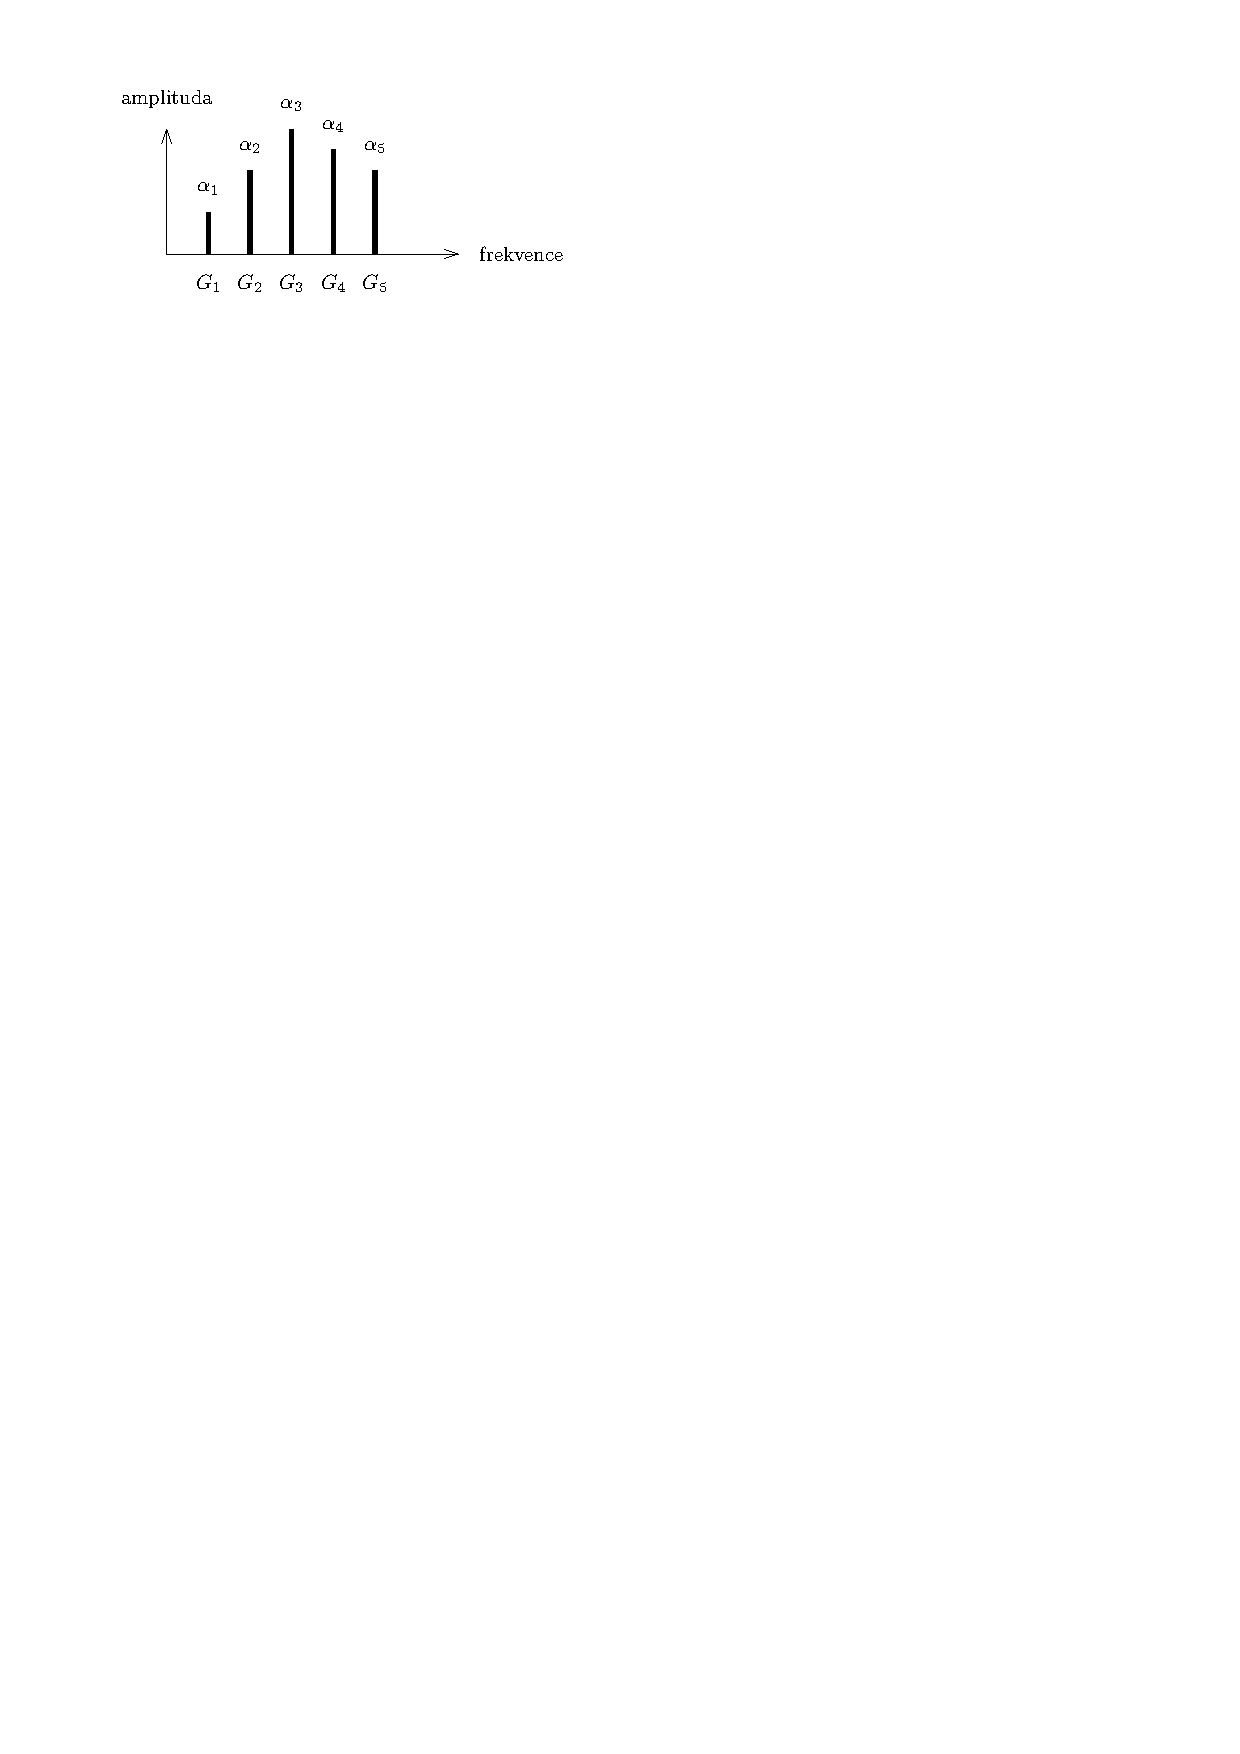
\includegraphics{diskretni-spektrum}
%\end{center}
%
%\subsection{Jaké typy konstitutivních modelů jsou potřebné pro úplný popis chování elastoplastického materiálu až do porušení při monotonním a~cyklickém zatěžování?}
%K~popisu pružně-plastického chování materiálu je nutné znát:
%\begin{enumerate}
%	\item Mezní podmínku plasticity
%	\begin{itemize}
%		\item Tresca
%		\item von Mises
%		\item Mohr-Coulomb
%		\item Drucker-Prager
%	\end{itemize}
%	\item Model plastického tečení -- křivka zpevnění pro jednoosou napjatost, příp. proporcionální zatěžování (flow curve)
%	\begin{itemize}
%		\item Ramberg-Osgood
%		\item Voce 4
%		\item Johnson-Cook -- viskoplastický model s~vlivem teploty
%		\item Norton -- model viskoplastického creepu
%	\end{itemize}
%	\item Model zpevnění materiálu
%	\begin{itemize}
%		\item Izotropní (nevhodné pro cyklické zatěžování)
%		\item Kinematické (popisuje Bauschingerův efekt) -- model Chaboche
%	\end{itemize}
%	\item Model plastického porušení
%	\begin{itemize}
%		\item Johnson-Cook
%		\item Bai-Wierzbicki
%	\end{itemize}
%\end{enumerate}
%
%\subsection{Jaký výsledek dostanete, jestliže v~podmínce plasticity Mohr-Coulomb (Drucker-Prager) zadané rovnicí pro redukované napětí použijete stejnou mez pružnosti pro tah a~tlak ($m=1$)?}
%
%\subsubsection{Podmínka plasticity Mohr-Coulomb}
%Představuje rozšíření Trescovy podmínky na materiály s~různou mezí kluzu v~tahu a~tlaku.
%Její redukované napětí je dáno rovnicí
%\begin{multline*}
%\sigma_\text{red}^\text{MC}
%= \frac{m+1}{2} \max\Big[
%\left|\sigma_\text{I} - \sigma_\text{II}\right| + K \left(\sigma_\text{I} + \sigma_\text{II}\right);
%\left|\sigma_\text{I} - \sigma_\text{III}\right| + K \left(\sigma_\text{I} + \sigma_\text{III}\right);\\
%\left|\sigma_\text{II} - \sigma_\text{III}\right| + K \left(\sigma_\text{II} + \sigma_\text{III}\right)
%\Big],
%\end{multline*}
%kde
%\begin{equation*}
%m = \frac{R_e^\text{tlak}}{R_e^\text{tah}}
%\qquad\text{a}\qquad
%K = \frac{m-1}{m+1}
%\end{equation*}
%a~v~Haighově prostoru hlavních napětí představuje pravidelný šestiboký jehlan.
%
%Pro $m=1$ dostaneme standardní tvar Trescovy podmínky.
%
%\subsubsection{Podmínka plasticity Drucker-Prager}
%Představuje de facto rozšíření Misesovy podmínky na materiály s~různou mezí kluzu v~tahu a~tlaku.
%Redukované napětí podle této podmínky je dáno rovnicí
%\begin{equation*}
%\sigma_\text{red}^\text{DP}
%= \frac{m-1}{2} \left(\sigma_\text{I} + \sigma_\text{II} + \sigma_\text{III}\right)
%+ \frac{m+1}{2} \sqrt{\frac{1}{2} \left[ (\sigma_\text{I}-\sigma_\text{II})^2 + (\sigma_\text{I}-\sigma_\text{III})^2 + (\sigma_\text{II}-\sigma_\text{II})^2 \right]}
%\end{equation*}
%nebo
%\begin{equation*}
%\sigma_\text{red}^\text{DP}
%= \frac{m-1}{2} I_1 + \frac{m+1}{2} \sqrt{I_1^2 - 3 I_2}
%\end{equation*}
%kde
%\begin{equation*}
%m = \frac{R_e^\text{tlak}}{R_e^\text{tah}}
%\end{equation*}
%a~v~Haighově prostoru hlavních napětí představuje kužel s~osou v~normále oktaedrické roviny.
%
%Pro $m=1$ dostaneme standardní tvar Misesovy podmínky.
%
%
%\subsection{Co je faktor triaxiality napětí? Jakých nabývá hodnot?}
%Střední napětí (hydrostatická -- kulová) složka tenzoru napětí nemá významný vliv na mez kluzu, ale má značný vliv na tvárné porušení. Jeho normalizovaná hodnota se nazývá faktor triaxiality napětí.
%
%Faktor triaxiality napětí $\eta$ je rozhodující pro přechod od tvárného ke křehkému porušení a~objevuje se spolu s~Lodeho parametrem v~některých mezních podmínkách, resp. konstitutivních modelech. Je dán poměrem kulové a~deviátorové části tenzoru napětí, konkrétně středního a~Misesova napětí, podle vztahu:
%\begin{equation}
%\eta = \frac{\sigma_s}{\sigma_\text{HMH}},
%\end{equation}
%kde
%\begin{description}
%	\item[$\sigma_s$] je střední napětí, reprezentující kulovou (hydrostatická) složku napjatosti,
%	\item[$\sigma_\text{HMH}$] je redukované napětí podle Misesovy podmínky plasticity (deviátorová složka napjatosti).
%\end{description}
%
%Z~vlastností uvedených složek napětí plyne, že $\eta$ je nulové pro smykovou napjatost (nulová střední složka napětí, čistý deviátor) a~dosahuje extrémních hodnot $+\infty/-\infty$ pro rovnoměrnou trojosou napjatost v~tahu (tlaku). 
%
%Změní-li se znaménko všech složek napětí, nezmění se velikost triaxiality, ale změní se jen znaménko faktoru triaxiality napětí.
%
%\subsection{Co je Lodeho parametr nebo úhel? V~jakém rozmezí se pohybují jeho hodnoty?}
%\subsubsection{Lodeho parametr}
%Dalším významným parametrem pro tvárné porušení vztaženým ke stavu napjatosti je Lodeho parametr $\mu$:
%\begin{equation}
%\mu = \frac{2 \sigma_2 - \sigma_1 - \sigma_3}{\sigma_1 - \sigma_3}
%\end{equation}
%
%Lodeho parametr nabývá hodnot v~intervalu $-1 \leq \mu \leq 1$ a~charakterizuje typ napjatosti z~hlediska polohy hlavního napětí $\sigma_2$ vůči $\sigma_1$ a~$\sigma_3$. Jeho význam se různí podle materiálů, je velký např. u~hliníkových slitin, u~ocelí pak při nízkých faktorech triaxiality napětí.
%\begin{figure}[H]\centering\begin{tabular}{lll}
%		\toprule
%		Název            &       $\mu$        &     Hlavní napětí      \\ \midrule
%		Smyková           &         $0$          &     $\sigma_3= -\sigma_1; \sigma_2=0$      \\
%		Jednoosá tahová       &         $-1$         &     $\sigma_1>0; \sigma_2= \sigma_3=0$     \\
%		Dvouosá tahová rovnoměrná  &         $1$          &     $\sigma_1=\sigma_2>0; \sigma_3=0$      \\
%		Jednoosá tlaková      &         $1$          &     $\sigma_3<0; \sigma_2= \sigma_1=0$     \\
%		Dvouosá tlaková rovnoměrná &         $-1$         &     $\sigma_3=\sigma_2<0; \sigma_1=0$      \\
%		Trojosá rovnoměrná     & Neurčitý výraz $0/0$ & $\sigma_1=\sigma_2=\sigma_3>0$\\
%		\bottomrule
%\end{tabular}\end{figure}
%
%\subsubsection{Lodeho úhel}
%Alternativním vyjádřením Lodeho parametru je Lodeho úhel $\theta$, který představuje normalizovaný arkustangens Lodeho parametru $\mu$; lze jej také vyjádřit pomocí normalizovaného třetího invariantu deviátoru napětí $\xi$:
%\begin{equation}
%\theta = \arctan\left(\frac{\mu}{\sqrt{3}}\right)
%\end{equation}
%nebo
%\begin{equation}
%\theta = -\frac{1}{3}\arcsin\left(\xi\right),
%\end{equation}
%kde
%\begin{equation*}
%\xi = \left(\frac{r}{\sigma_\text{Mises}}\right)^3
%= \frac{27}{2} \frac{\det \bm{S}}{\sigma_\text{Mises}^3},
%\end{equation*}
%přičemž
%\begin{equation*}
%r = \sqrt[3]{\frac{9}{2} \bm{S}\cdot\bm{S}\!:\!\bm{S}}
%= \sqrt[3]{\frac{27}{2} \det\bm{S}}
%= \sqrt[3]{\frac{27}{2} (\sigma_1-\sigma_m)(\sigma_2-\sigma_m)(\sigma_3-\sigma_m)},
%\end{equation*}
%kde
%\begin{description}
%	\item[$\bm{S}$] reprezentuje deviátor tenzoru napětí,
%	\item[$\sigma_\text{Mises}$] je střední (hydrostatická) složka napětí,
%	\item[$\sigma_m$] je redukované napětí podle von Misesovy podmínky plasticity.
%\end{description}
%
%Lodeho úhel nabývá hodnot v~intervalu $-\frac{\pi}{6} \leq \theta \leq \frac{\pi}{6}$, normalizovaný třetí invariant deviátoru napětí je v~intervalu $-1 \leq \xi \leq 1$. 
%
%Především v~mezních podmínkách porušení má faktor triaxiality napětí a~Lodeho parametr velký význam, protože ovlivňují vznik porušení. Experimentální ověřování mezních podmínek je třeba proto provádět při různých hodnotách těchto parametrů; lze je měnit typem namáhání vzorku (tah, tlak, biaxiální tah-tlak, krut, různé jejich kombinace) nebo změnou jeho geometrie (poloměru vrubu).
%
%\subsection{Určete faktor triaxiality napětí pro zadanou napjatost.}
%\begin{figure}[H]\centering\begin{tabular}{lll}\toprule
%		Název & $\eta$ & Hlavní napětí\\ \midrule
%		Smyková & $0$ & $\sigma_3 = -\sigma_1; \sigma_2 = 0$\\
%		Dvouosá s~opačnými znam. hl. napětí & $0< \eta < \tfrac{1}{3}$ & $0 < |\sigma_3| = -\sigma_3 < \sigma_1; \sigma_2 = 0$\\
%		Jednoosá tahová & $\eta = \tfrac{1}{3}$ & $\sigma_1 > 0; \sigma_2 = \sigma_3 = 0$\\
%		Dvouosá tahová nerovnoměrná & $\tfrac{1}{3} < \eta < \tfrac{2}{3}$ & $0 < \sigma_2 < \sigma_1; \sigma_3 = 0$\\
%		Dvouosá tahová rovnoměrná & $\eta = \tfrac{2}{3}$ & $\sigma_1 = \sigma_2 > 0; \sigma_3 = 0$\\
%		Trojosá tahová polorovnoměrná & $\eta > \tfrac{2}{3}$ & $0 < \sigma_3 < \sigma_1 = \sigma_2$\\
%		Trojosá tahová polorovnoměrná & $\eta = 1$ & $0 < \sigma_1 = \sigma_2; \sigma_3 = \tfrac{\sigma_1}{4}$\\
%		Trojosá tahová polorovnoměrná & $\eta = \tfrac{10}{6} \approx 1\!,67$ & $0 < \sigma_1 = \sigma_2; \sigma_3 = \tfrac{\sigma_1}{2}$\\
%		Trojosá tahová rovnoměrná & $\eta \rightarrow \infty$ & $\sigma_1 = \sigma_2 = \sigma_3 > 0$\\
%		\bottomrule\end{tabular}
%	\caption{Závislost součinitele triaxiality napětí $\eta$ na typu napjatosti}
%\end{figure}
%
%\begin{figure}[H]\centering\begin{tabular}{lll}\toprule
%		Název & $\eta$ & Hlavní napětí\\ \midrule
%		Smyková & $0$ & $\sigma_3 = -\sigma_1; \sigma_2 = 0$\\
%		Dvouosá s opačnými znam. hl.  napětí & $0 > \eta > -\tfrac{1}{3}$ & $\sigma_1 < |\sigma_3|; \sigma_2 = 0; \sigma_3 < 0$\\
%		Jednoosá tlaková & $\eta= -\tfrac{1}{3}$ & $\sigma_1 = \sigma_2 = 0; \sigma_3 < 0$\\
%		Dvouosá tlaková nerovnoměrná & $-\tfrac{1}{3} > \eta > -\tfrac{2}{3}$ & $\sigma_1 = 0; \sigma_3 < \sigma_2 < 0$\\
%		Dvouosá tlaková rovnoměrná & $\eta = -\tfrac{2}{3}$ & $\sigma_1 = 0; \sigma_2 = \sigma_3 < 0$\\
%		Trojosá tlaková polorovnoměrná & $\eta < -\tfrac{2}{3}$ & $0 > \sigma_1 > \sigma_2 = \sigma_3$\\
%		Trojosá tlaková polorovnoměrná & $\eta = -1$ & $\sigma_1 = \tfrac{\sigma_3}{4}; \sigma_2 = \sigma_3 < 0$\\
%		Trojosá tlaková polorovnoměrná & $\eta= -\tfrac{10}{6} \approx -1\!,67$ & $\sigma_1 = \tfrac{\sigma_3}{2}; \sigma_2 = \sigma_3 < 0$\\
%		Trojosá tlaková rovnoměrná & $\eta \rightarrow -\infty$ & $\sigma_1 = \sigma_2 = \sigma_3 < 0$\\
%		\bottomrule\end{tabular}
%	\caption{Závislost součinitele triaxiality napětí $\eta$ na typu napjatosti (tlakové)}
%\end{figure}